% ============================================================
% 直流回路（テスターによる電気測定） 本文
% 担当の先生はこのファイルと figures/ だけを編集してください。
% 図のラベルは fig:tester-○○ の形にしてください（他テーマとの重複防止）。
% ============================================================
\graphicspath{{contents/01_tester/figures/}}

\experimenttitle{直流回路（テスターによる電気測定）}

% ============================================================
\section{目的}

デジタルテスターは，電圧や抵抗などを手軽に測定できる計測器で，電気回路の実験や電気機器の点検に欠かせない道具です。本実験では，デジタルテスターの基本的な使い方を学び，乾電池，USB（Universal Serial Bus）ポート，ACアダプタ，コンセントなど家庭にあるさまざまな電源の電圧を測定して，電圧源の特徴を理解します。さらに，鉛筆で紙に書いた線を抵抗体として利用し，線の長さ・幅・形状と抵抗値の関係を調べます。本実験の概要を\cref{fig:tester-overview}に示します。

\begin{figure}[htbp]
  \vspace{5mm}
  \centering
  % 本実験の概要図（TikZ で作成。原本にはない図）
  \begin{tikzpicture}[
      font=\small,
      lbl/.style={font=\sffamily\gtfamily\footnotesize, align=center},
      ttl/.style={font=\sffamily\gtfamily\bfseries\small, text=EGMain},
      tester/.pic={
        \draw[fill=black!75, rounded corners=3pt] (-0.6,-1.0) rectangle (0.6,1.0);
        \draw[fill=black!8] (-0.45,0.35) rectangle (0.45,0.8);
        \node[font=\scriptsize\bfseries] at (0,0.575) {1.50};
        \draw[fill=black!40, draw=black!20] (0,-0.2) circle (0.3);
        \draw[white, line width=0.8pt] (0,-0.2) -- (0.2,0.0);
        \fill[red!70!black] (-0.3,-0.78) circle (0.08);
        \fill[black] (0.3,-0.78) circle (0.08);
        \draw[black!20] (0.3,-0.78) circle (0.08);
      },
    ]
    % ===== 左：電圧を測る =====
    \draw[EGMain, rounded corners=4pt] (-0.3,-2.1) rectangle (7.3,2.2);
    \node[ttl, anchor=north west] at (-0.1,2.1) {電圧を測る（実験1，2）};
    \pic at (0.8,0.1) {tester};
    \node[lbl] at (0.8,-1.45) {デジタル\\テスター};
    % プローブ
    \draw[red!70!black, line width=1pt] (0.5,-0.68) .. controls (1.4,-1.6) and (1.7,1.3) .. (2.85,0.9);
    \fill[red!70!black] (2.85,0.9) circle (0.06);
    \draw[black, line width=1pt] (1.1,-0.68) .. controls (1.6,-1.1) and (2.2,-0.9) .. (2.85,-0.5);
    \fill[black] (2.85,-0.5) circle (0.06);
    % 乾電池
    \begin{scope}[shift={(2.85,0.15)}]
      \draw[fill=black!8, rounded corners=1pt] (-0.25,-0.6) rectangle (0.25,0.6);
      \fill[black!55] (-0.25,0.35) rectangle (0.25,0.6);
      \draw[fill=black!35] (-0.08,0.6) rectangle (0.08,0.7);
      \node[lbl] at (0,-1.25) {乾電池};
    \end{scope}
    % USB
    \begin{scope}[shift={(4.0,0.15)}]
      \draw[fill=black!8, rounded corners=2pt] (-0.4,-0.3) rectangle (0.4,0.3);
      \draw[fill=black!60] (-0.25,-0.08) rectangle (0.25,0.12);
      \node[lbl] at (0,-1.25) {USB};
    \end{scope}
    % ACアダプタ
    \begin{scope}[shift={(5.2,0.15)}]
      \draw[fill=black!15, rounded corners=2pt] (-0.35,-0.45) rectangle (0.35,0.45);
      \draw[line width=1.2pt, black!70] (0,-0.45) -- (0,-0.7);
      \node[lbl] at (0,-1.25) {AC\\アダプタ};
    \end{scope}
    % コンセント
    \begin{scope}[shift={(6.5,0.15)}]
      \draw[fill=white, rounded corners=4pt] (-0.4,-0.5) rectangle (0.4,0.5);
      \fill[black!70] (-0.14,0.0) rectangle (-0.08,0.25);
      \fill[black!70] (0.08,0.0) rectangle (0.14,0.25);
      \node[lbl] at (0,-1.25) {コンセント\\（交流）};
    \end{scope}
    % ===== 右：抵抗を測る =====
    \draw[EGMain, rounded corners=4pt] (7.7,-2.1) rectangle (15.0,2.2);
    \node[ttl, anchor=north west] at (7.9,2.1) {抵抗を測る（実験3，4）};
    \pic at (8.7,0.1) {tester};
    \node[lbl] at (8.7,-1.45) {デジタル\\テスター};
    % 方眼紙と鉛筆の線
    \begin{scope}[shift={(10.0,-1.2)}]
      \fill[EGSub] (0,0) rectangle (4.6,2.4);
      \draw[step=0.2, EGMain!25, very thin] (0,0) grid (4.6,2.4);
      \draw[EGMain!60] (0,0) rectangle (4.6,2.4);
      \fill[black!80] (0.4,0.9) rectangle (4.2,1.25);
      \node[lbl, anchor=north] at (2.3,-0.05) {方眼紙に鉛筆で書いた線};
    \end{scope}
    % 鉛筆
    \begin{scope}[shift={(13.3,0.75)}, rotate=25]
      \fill[orange!80!black] (0,0) rectangle (1.4,0.18);
      \fill[yellow!60!orange] (-0.3,0) -- (0,0) -- (0,0.18) -- (-0.3,0.09) -- cycle;
      \fill[black] (-0.3,0.09) -- (-0.2,0.04) -- (-0.2,0.14) -- cycle;
    \end{scope}
    % プローブ
    \draw[red!70!black, line width=1pt] (8.4,-0.68) .. controls (9.2,-1.4) and (10.0,-0.6) .. (10.6,-0.12);
    \fill[red!70!black] (10.6,-0.12) circle (0.06);
    \draw[black, line width=1pt] (9.0,-0.68) .. controls (10.5,-1.6) and (12.6,-0.9) .. (13.6,-0.12);
    \fill[black] (13.6,-0.12) circle (0.06);
  \end{tikzpicture}
  \caption{本実験の概要}
  \label{fig:tester-overview}
\end{figure}


% ============================================================
\section{原理}

% ------------------------------------------------------------
\subsection{身の周りの電圧}

私たちの身の回りには様々な電源が存在し，乾電池（約\SI{1.5}{V}），USBポート（約\SI{5}{V}），ACアダプタ（約\SI{12}{V}），コンセント（約\SI{100}{V}，交流）など，それぞれ異なる電圧を持っています。

\important{乾電池}は，内部の化学反応によって化学エネルギーを電気エネルギーに変換する直流電源です。
一般的なアルカリ乾電池は，1本あたりおよそ\SI{1.5}{V}の電圧を生じ，リモコンや時計，懐中電灯など，身の周りのさまざまな電気機器に利用されています。

\important{USBポート}は，通常\SI{5}{V}の直流電圧を供給するように設計されており，内部には電圧を安定化するための電源回路が組み込まれています。そのためPCや充電器のUSB端子は通常，安定した直流電圧を供給しますが，接続する機器が大きな電流を要求した場合や規格に合わない使い方をした場合には，電圧が下がったり，安全のために保護回路が働いたりします。

\important{ACアダプタ}（AC-DCアダプタ）は，家庭用コンセントから供給される交流\SI{100}{V}を電子回路によって直流電圧に変換する装置です。ノートパソコンやルータ，電子工作用機器など，多くの電子機器で利用されています。出力電圧は機器によって異なり，\SI{5}{V}，\SI{9}{V}，\SI{12}{V}，\SI{24}{V}などさまざまです。本実験で使用するACアダプタは約\SI{12}{V}の直流電圧を出力します。

\important{コンセント}は，家庭や教室で使われている商用電源であり，日本では交流\SI{100}{V}（周波数は地域により\SI{50}{Hz}または\SI{60}{Hz}）を供給しています。乾電池やUSBポートに比べて大きな電圧と電力を取り出すことができ，多くの電気製品を直接動かすことができます。一方で，高電圧であるため感電の危険があり，測定の際には注意が必要です。また，テスターで測定するときは測定モードを交流電圧（ACV）に切り替える必要があります。

このように，電源の種類によって，電圧の大きさや直流・交流の違い，電圧の安定性が異なります。本実験では，乾電池，USBポート，ACアダプタ，コンセントの電圧を測定することで，用途に応じた電源の違いを学びます（実験1）。

% ------------------------------------------------------------
\subsection{電源の電圧降下と等価回路}

電源が電流を供給する能力には限界があり，実際に電流を取り出すと，電源の端子間の電圧（\important{端子電圧}）は，何もつながない状態で測定される電圧（\important{開放電圧}）よりも低下してしまいます。このような電圧降下を説明するために，電源は「理想的な電圧源に対して直列に小さな抵抗が入っている」と考えて表すことができます。乾電池の場合の例を\cref{fig:tester-battery}に示します。この直列の抵抗を\important{内部抵抗}（あるいは\important{出力インピーダンス}）と呼びます。

\begin{figure}[htbp]
  \centering
  \begin{circuitikz}
    % 乾電池（点線の枠の中）
    \draw[dashed, EGMain, rounded corners=3pt] (-2.4,-0.5) rectangle (3.0,3.2);
    \node[font=\sffamily\gtfamily\small, text=EGMain, anchor=south west] at (-2.4,3.22) {乾電池};
    \draw (0,0) to[battery1, l={起電力 $E$}] (0,2.4)
          to[R, l={内部抵抗 $r$}, i>_=$I$] (2.6,2.4) to[short, -o] (3.0,2.4);
    \draw (0,0) to[short, -o] (3.0,0);
    % 負荷
    \draw (3.0,2.4) -- (5.3,2.4) to[R, l_=$R$] (5.3,0) -- (3.0,0);
    \draw[-latex] (3.35,0.2) -- node[right, align=left] {端子\\電圧 $V$} (3.35,2.2);
    \node[font=\sffamily\gtfamily\footnotesize, align=center, anchor=west] at (5.65,1.2) {負荷\\（抵抗器）};
  \end{circuitikz}
  \caption{乾電池の等価回路}
  \label{fig:tester-battery}
\end{figure}

理想的な電圧源の電圧（起電力）を $E$，内部抵抗を $r$，電源から取り出す電流を $I$ とすると，端子電圧 $V$ は
\begin{equation}
  V = E - rI
  \label{eq:tester-terminal}
\end{equation}
となり，電流が大きいほど端子電圧は低くなります。本実験では，乾電池に負荷抵抗を接続して端子電圧の変化を調べることで，内部抵抗の存在を体験的に理解します（実験2）。

% ------------------------------------------------------------
\subsection{炭素材料と鉛筆芯}

本実験では，鉛筆で紙に描いた線の抵抗を測定します。鉛筆の線は一見ただの黒い跡に見えますが，実際には電気を通す性質をもっています。これは，鉛筆の芯に含まれる炭素材料の黒鉛（グラファイト）が導電性を持つためです。

炭素には，ダイヤモンド・グラファイト・グラフェン・カーボンナノチューブなど多様な同素体が存在します（\cref{fig:tester-carbon}）。これらはすべて炭素原子だけからなりますが，原子の結合の仕方が異なるために性質が大きく変化します。たとえばダイヤモンドは電気を通さない絶縁体である一方，グラファイトやグラフェンは良好な導電性を示します。

\begin{figure}[htbp]
  \centering
  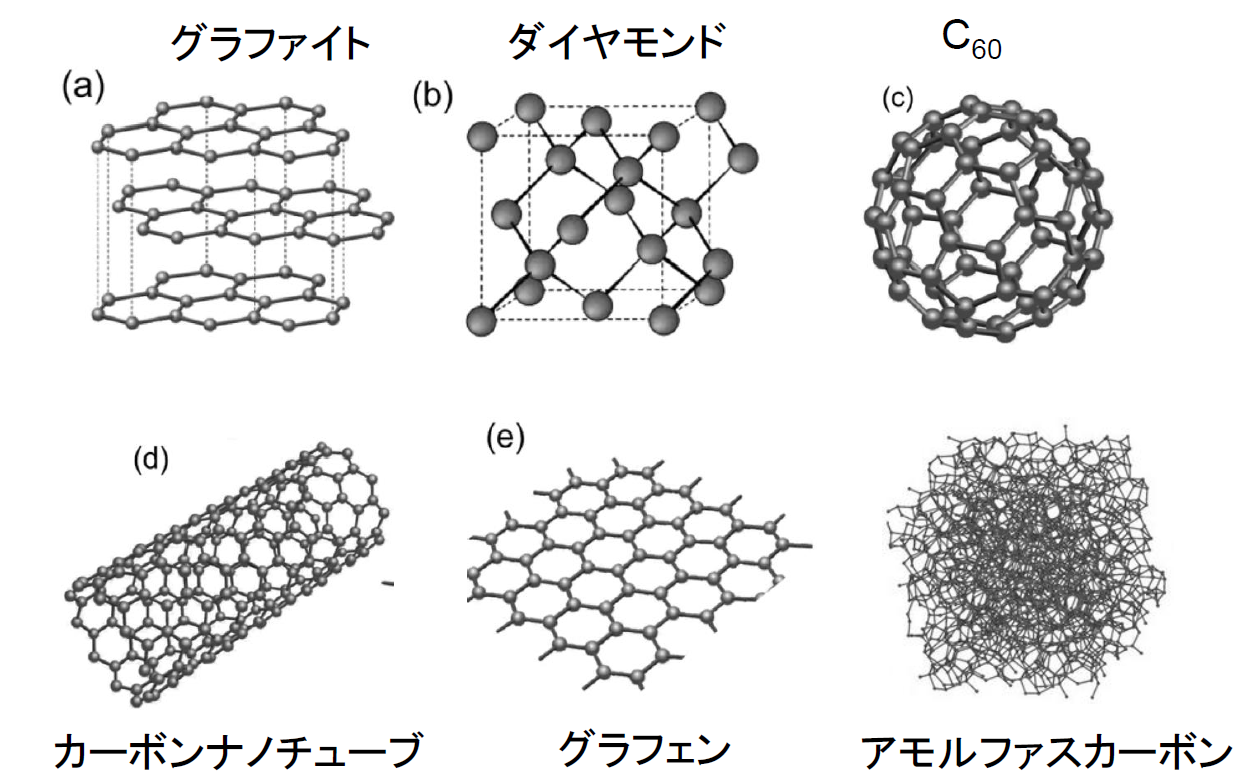
\includegraphics[width=0.8\linewidth]{tester_carbon.png}
  \caption{いろいろな炭素材料}
  \label{fig:tester-carbon}
\end{figure}

鉛筆の芯は，グラファイトと粘土を混ぜ合わせて焼き固めたものです。グラファイトの割合が多いほど芯は柔らかく（B系統），導電性も高くなります。逆に粘土の割合が多いと芯は硬く（H系統），導電性は低くなります。したがって，鉛筆の硬度によって電気の通りやすさが異なります。紙に鉛筆で線を引くと，グラファイトの微小片が紙の表面に付着し，それらが互いに接触して電流の通り道を形成します（\cref{fig:tester-pencil}）。この経路の長さが長くなれば抵抗は大きくなり，幅が広くなれば抵抗は小さくなります。また，塗り方の濃さや重ね塗り，紙の表面の形状の変化によっても，黒鉛片どうしのつながりが変化して抵抗値が変動します。

\begin{figure}[htbp]
  \centering
  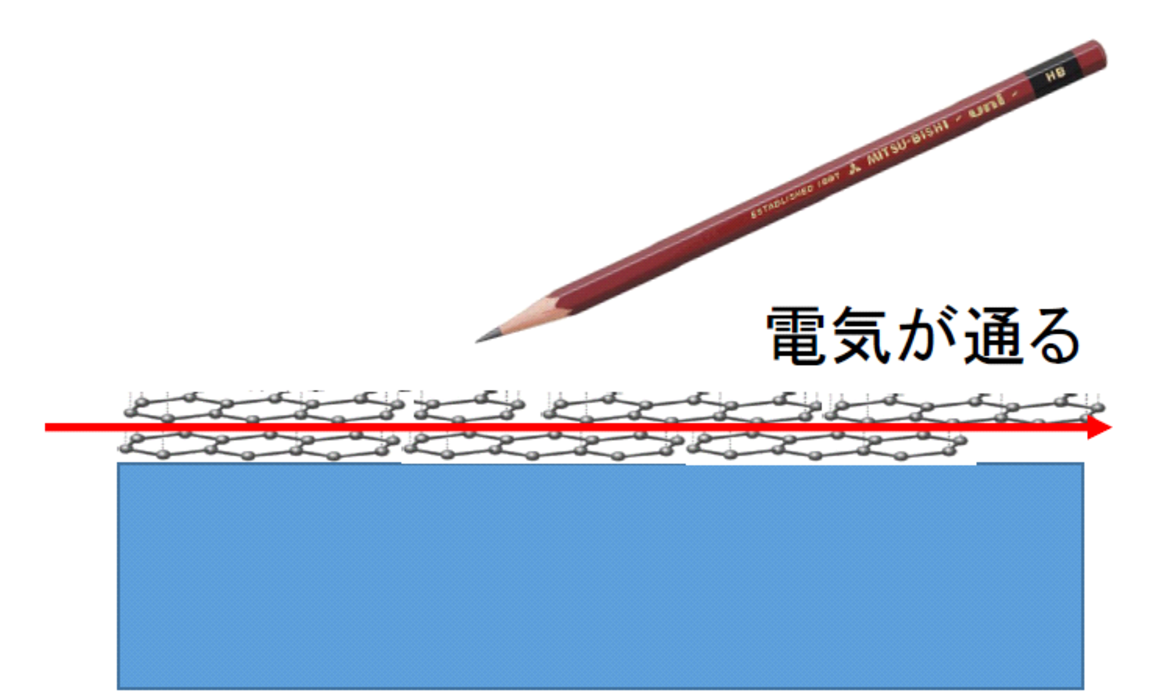
\includegraphics[width=0.5\linewidth]{tester_pencil_line.pdf}\hfill
  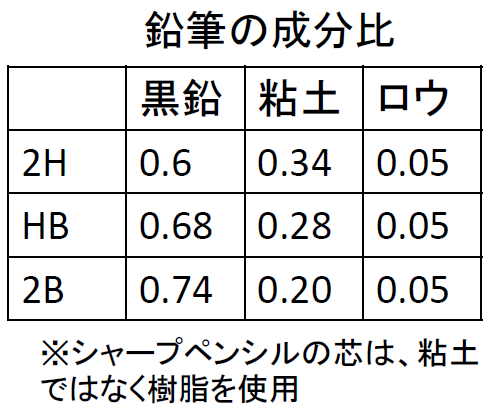
\includegraphics[width=0.42\linewidth]{tester_pencil_composition.png}
  \caption{鉛筆芯の特性}
  \label{fig:tester-pencil}
\end{figure}


% ============================================================
\section{使用器具と使い方}

\begin{equipment}
\begin{itemize}
  \item デジタルテスター
  \item 乾電池・電池ボックス
  \item 抵抗（\SI{100}{\ohm}，\SI{200}{\ohm}，\SI{1}{k\ohm}）
  \item ブレッドボード・リード線
  \item USB充電器，コンセント，ACアダプタ
  \item 鉛筆（2Bなど濃いものが望ましい）
  \item 方眼紙
\end{itemize}
\end{equipment}

% ------------------------------------------------------------
\subsection{デジタルテスターの使い方}

\begin{figure}[htbp]
  \centering
  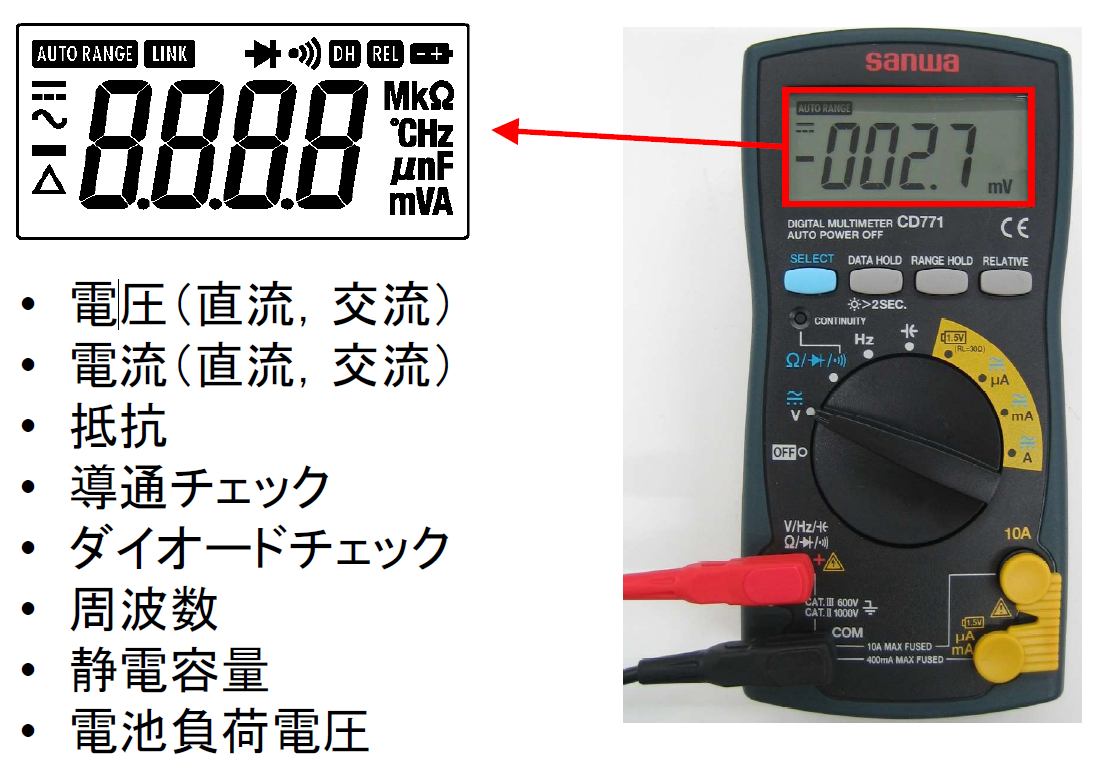
\includegraphics[width=0.72\linewidth]{tester_multimeter.png}
  \caption{デジタルテスター}
  \label{fig:tester-multimeter}
\end{figure}

デジタルテスターは，電気回路の基本的な特性を測定するための装置です。主に電圧（直流・交流），電流（直流・交流），抵抗の測定に用いられるほか，導通チェックやダイオードチェック，静電容量や周波数の測定機能を備えています（\cref{fig:tester-multimeter}）。

\begin{figure}[htbp]
  \centering
  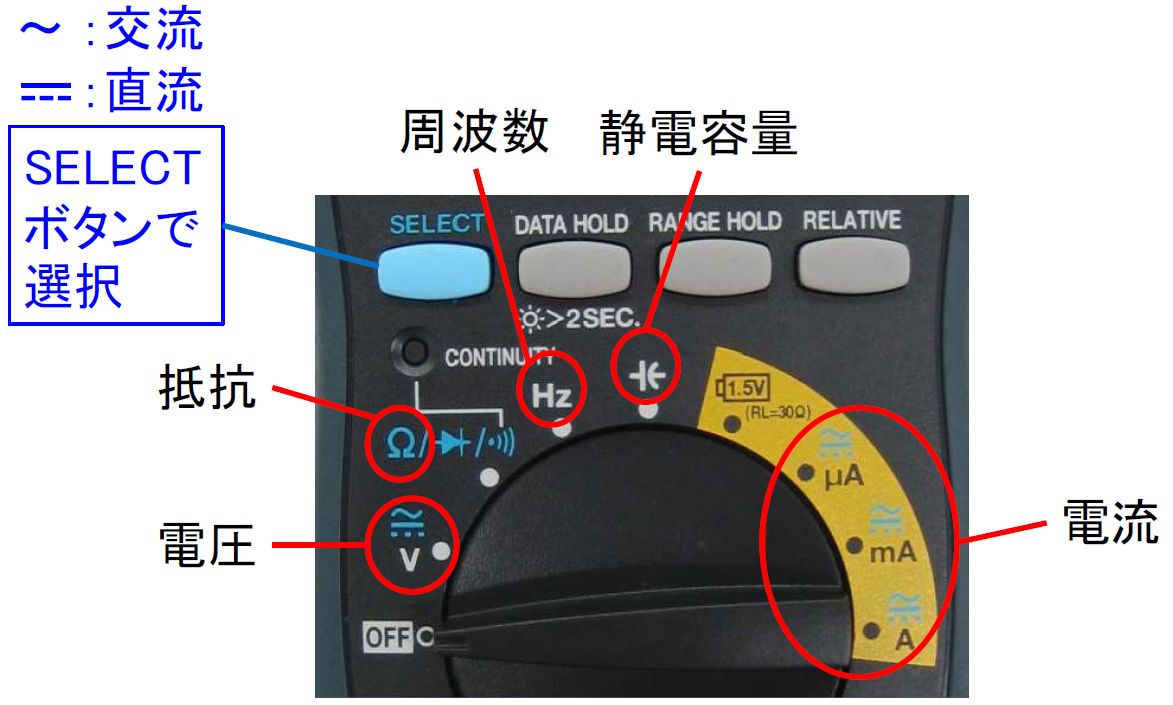
\includegraphics[width=0.72\linewidth]{tester_modes.png}
  \caption{デジタルテスターの測定モード}
  \label{fig:tester-modes}
\end{figure}

本実験では，電圧測定と抵抗測定を中心に使用します。\cref{fig:tester-modes}に示すように，テスターの前面には測定モードを切り替えるためのダイヤルがあり，測定対象に応じて「直流電圧」「交流電圧」「抵抗」などを選択します。直流と交流は表示記号が異なり，直線（―）は直流を，波形（～）は交流を意味します。さらに一部の機種では「SELECT」ボタンを押すことで，同じ測定レンジ内で直流と交流を切り替えることができます。

プローブは赤と黒の2本があり，黒は常に「COM」端子に接続し，赤は測定対象に応じて「V/$\Omega$」端子（電圧・抵抗測定用）や「A」端子（電流測定用）に差し込みます。\wave{誤った端子に差し込んだまま測定すると，ヒューズが切れるなど故障の原因となるため注意が必要です。}測定時には，対象の電気回路の性質に応じて以下の点に注意してください。

\begin{itemize}
  \item \important{電圧測定：}回路を切り離さず，測定したい部分の両端にプローブを当てます。直流の場合は極性（赤がプラス，黒がマイナス）を確認します。
  \item \important{抵抗測定：}\wave{必ず電源を外した状態で行います。}電源が入ったまま抵抗を測定すると誤った値が表示されるだけでなく，テスターを破損させる恐れがあります。また，大きな抵抗値（およそ数百\si{k\ohm}以上）を測定する場合には，テスター内部の構造（内部抵抗）の影響によって正しい値が得られないことがあります。テスターは理想的な計測器ではなく，有限の内部抵抗を持っているためです。これにより実際にどのような誤差が生じるか，また内部抵抗がどのように影響するかについては，2年生で行う電気電子工学実験IIで詳しく取り扱います。
  \item \important{交流測定（コンセント等）：}高電圧を扱うため，\wave{必ず教員の立ち会いのもとで操作し，プローブの金属部分には触れないようにしてください。}
\end{itemize}

このように，デジタルテスターは正しく操作すれば非常に多用途かつ便利な計測器ですが，不注意に扱うと危険や誤測定につながります。したがって，測定対象に合わせたダイヤル設定，端子接続，プローブの扱い方を理解し，安全に使用することが重要です。

% ------------------------------------------------------------
\subsection{ブレッドボードの使い方}

ブレッドボードは，電子回路の試作や学習に広く用いられる基板です。はんだ付けを行わずに部品やリード線を差し込むだけで回路を組むことができるため，初心者でも安全に回路実験を行えるのが特徴です。内部は金属のクリップで構成されており，穴の並び方によって導通の範囲が決まっています。一般的なブレッドボードでは，以下のような規則で電気的に接続されています。

\begin{figure}[htbp]
  \centering
  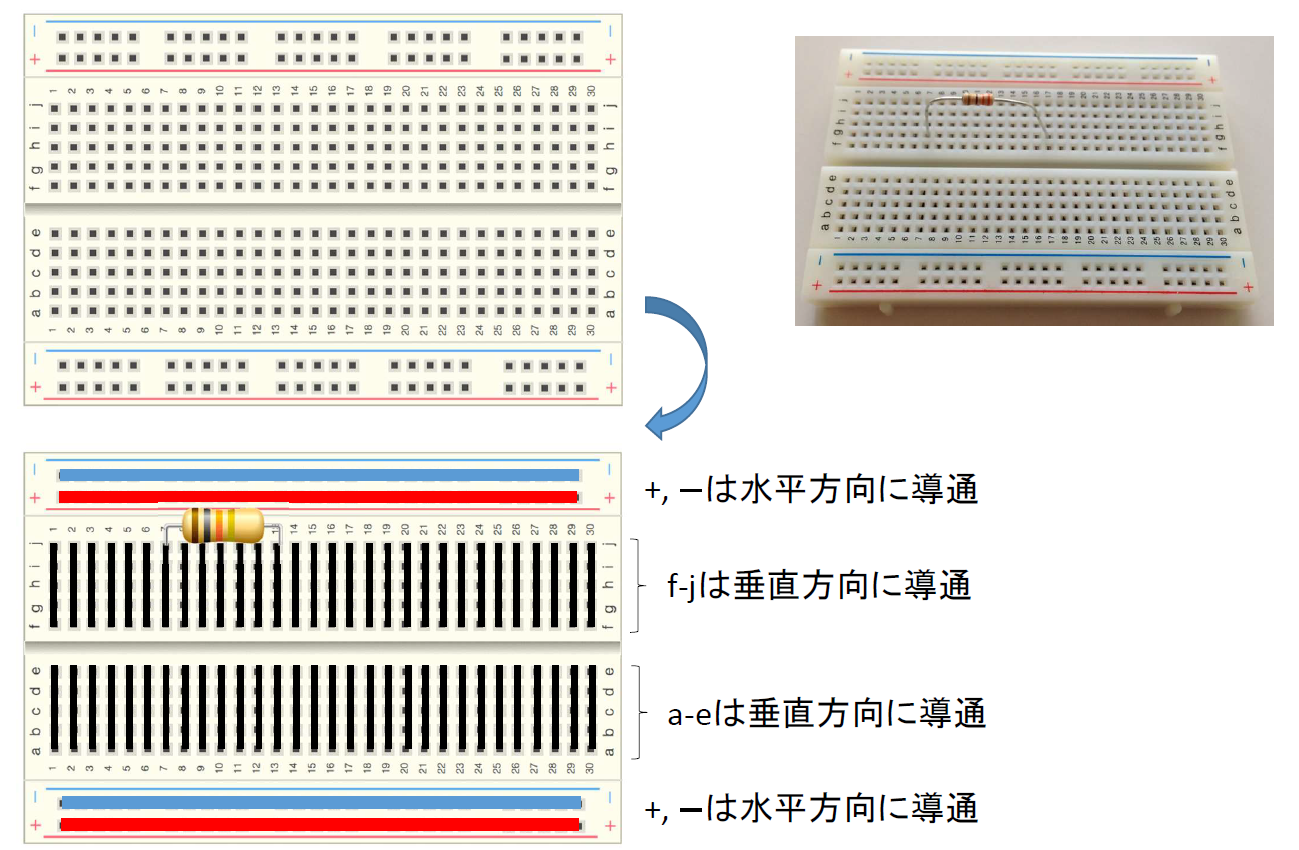
\includegraphics[width=0.8\linewidth]{tester_breadboard.png}
  \caption{ブレッドボード}
  \label{fig:tester-breadboard}
\end{figure}

\begin{itemize}
  % 原文は「図２」だが，ブレッドボードの図を指すため図3（fig:breadboard）に修正
  \item \important{中央部分（\cref{fig:tester-breadboard} a〜e列，f〜j列）：}縦方向に5つの穴がつながっています。ここに抵抗や素子のリードを差し込むと，同じ列内で電気的に接続されます。
  \item \important{両側の電源ライン（$+$，$-$の表示付き）：}横方向に長く連続して導通しています。電源のプラスとマイナスをここに配線しておくことで，どの位置からでも電源を取り出せます。
\end{itemize}

実際に回路を組むときには，乾電池ボックスなどの電源を$+$ラインと$-$ラインに接続し，抵抗やリード線を中央部分に差し込んで回路を構成します。抵抗を直列に接続する場合は，異なる縦列にまたがるように配置し，並列接続にする場合は同じ縦列に差し込みます。

% ------------------------------------------------------------
\subsection{抵抗器の表示}

\begin{figure}[htbp]
  \centering
  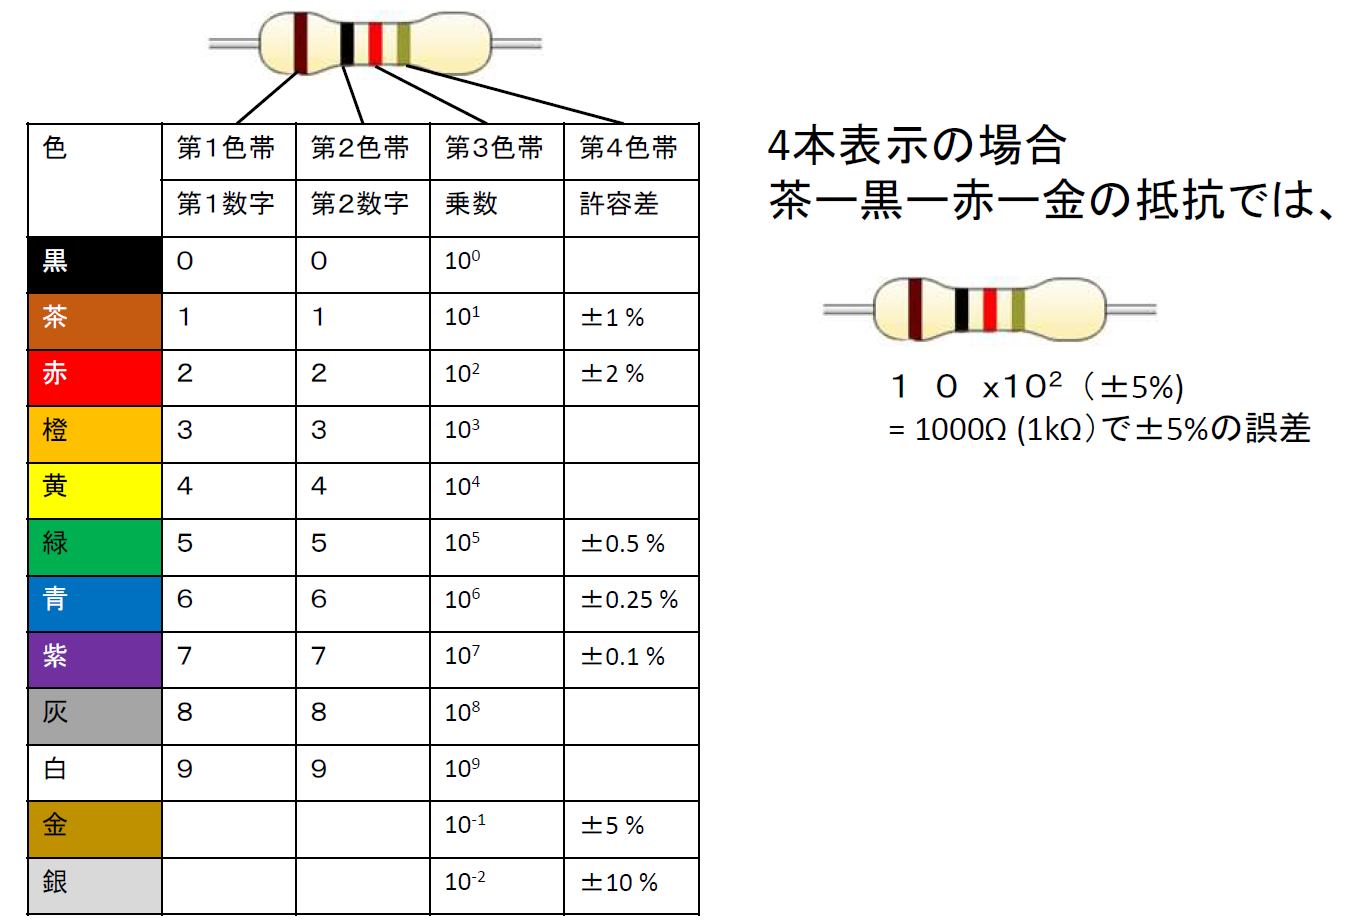
\includegraphics[width=0.8\linewidth]{tester_colorcode.png}
  \caption{カラーコードによる抵抗値の表示方法（JIS C 5062）}
  \label{fig:tester-colorcode}
\end{figure}

市販の抵抗器には抵抗値が印刷されていないものも多く，その場合は「カラーコード」によって値が示されています。\cref{fig:tester-colorcode}に示すように，4本表示の場合には，第1帯および第2帯がそれぞれ抵抗値の第1数字および第2数字を表し，第3帯が乗数（10の何乗を掛けるか），第4帯が許容差（誤差範囲）を表します。例えば「茶--黒--赤--金」の場合は
\begin{itemize}
  \item 第1帯（茶）＝1
  \item 第2帯（黒）＝0
  \item 第3帯（赤）＝$\times 100$
  \item 第4帯（金）＝許容差 $\pm\SI{5}{\percent}$
\end{itemize}
となり，抵抗値は $10\times 100 = \SI{1000}{\ohm}$（\SI{1}{k\ohm}）$\pm\SI{5}{\percent}$ となります。実験では，\SI{100}{\ohm}，\SI{200}{\ohm}，\SI{1}{k\ohm}の抵抗を使用します。

% ============================================================
\section{実験方法}

% ------------------------------------------------------------
\subsection{実験1：身近な電圧を測る}

\begin{procedure}[label=\textbf{1.\arabic*}, ref=1.\arabic*, leftmargin=*, labelsep=0.8em]
  \item テスターを直流電圧（DCV）に設定し，黒プローブをCOM，赤プローブをV/$\Omega$端子へ接続します。
  \item \important{乾電池：}電池ボックスの$+$と$-$にプローブを当て，端子電圧 $V_0$ を測定します。
  \item \important{USBポート：}通常のUSBコネクタは端子間が狭く，\wave{テスターのプローブを直接当てるとショートの危険があります。}そのため，本実験では，あらかじめ準備した「測定用USBケーブル」を使用し，端子部分にプローブを当てて，USB電圧を測定します。
  \item \important{ACアダプタ：}ACアダプタの出力端子にプローブを当て，出力電圧を測定します。
  \item \important{コンセント（AC）：}テスターを交流電圧（ACV）に切り替えます（プローブ端子の差し替えは不要です）。\wave{教員立会いのもと}，商用電源の電圧を測定します。
\end{procedure}

% ------------------------------------------------------------
\subsection{実験2：負荷をつないだときの電圧}

\begin{procedure}[label=\textbf{2.\arabic*}, ref=2.\arabic*, leftmargin=*, labelsep=0.8em]
  \item テスターを直流電圧（DCV）に戻します。
  \item ブレッドボード上で乾電池と\SI{1}{k\ohm}の抵抗を直列に接続し，乾電池の両端の電圧 $V_{1\,\mathrm{k\Omega}}$ を測定します。
  \item 抵抗を\SI{200}{\ohm}や\SI{100}{\ohm}に取り替え，同様に乾電池の両端の電圧 $V_{200\,\Omega}$ および $V_{100\,\Omega}$ をそれぞれ測定します。
  \item それぞれの抵抗値・電圧値をまとめます。さらに，抵抗値から電流を計算し，電流と電圧の関係を確認します。
\end{procedure}

% ------------------------------------------------------------
\subsection{実験3：鉛筆で書いた線の長さ・幅と抵抗値の関係}

\begin{figure}[htbp]
  \centering
  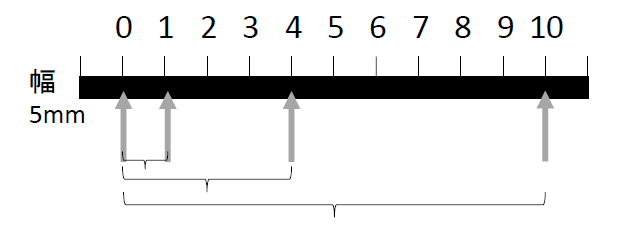
\includegraphics[width=0.47\linewidth]{tester_expC_5mm.png}\hfill
  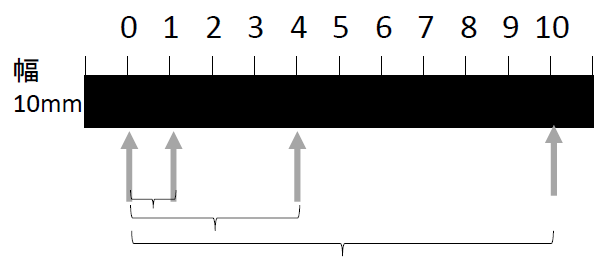
\includegraphics[width=0.47\linewidth]{tester_expC_10mm.png}
  \caption{鉛筆で書いた線の長さ・幅と抵抗値の関係の実験}
  \label{fig:tester-exp3}
\end{figure}

\begin{procedure}[label=\textbf{3.\arabic*}, ref=3.\arabic*, leftmargin=*, labelsep=0.8em]
  \item テスターを抵抗測定（$\Omega$）に設定し，黒プローブをCOM，赤プローブをV/$\Omega$端子へ接続します（プローブの差し替えは不要です）。
  \item 方眼紙に鉛筆で，線幅\SI{5}{mm}，長さ\SI{12}{cm}の線を書き，内部を濃く，均等に塗りつぶします（\cref{fig:tester-exp3}左）。
  \item 長さ\SI{12}{cm}のうち内部\SI{10}{cm}の部分について，\SI{1}{cm}ごとに長さと抵抗の関係を測定します。この際，塗りムラや濃さにより抵抗値が変わり得るので，測定値を観察しながら必要に応じて線を塗り足すなど工夫してかまいません。
  \item 次に，線幅を\SI{10}{mm}として同様の実験を行います（\cref{fig:tester-exp3}右）。
\end{procedure}

% ------------------------------------------------------------
\subsection{実験4：鉛筆で書いた線の曲げ方向と抵抗値の関係}

\begin{figure}[htbp]
  \centering
  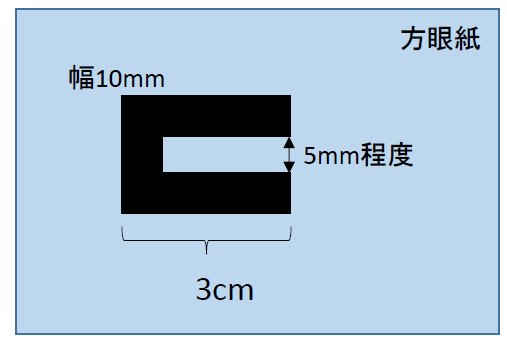
\includegraphics[width=0.47\linewidth]{tester_expD_cut.png}\hfill
  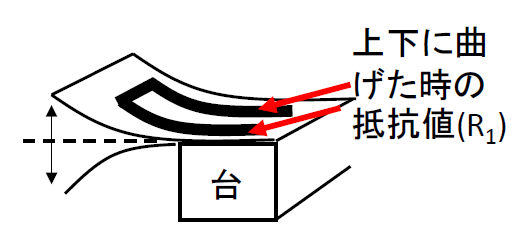
\includegraphics[width=0.47\linewidth]{tester_expD_bend.png}
  \caption{鉛筆で書いた線の曲げ方向と抵抗値の関係の実験}
  \label{fig:tester-exp4}
\end{figure}

\begin{procedure}[label=\textbf{4.\arabic*}, ref=4.\arabic*, leftmargin=*, labelsep=0.8em]
  \item 方眼紙に鉛筆で，幅\SI{10}{mm}，間隔\SI{5}{mm}，長さ\SI{3}{cm}程度のコ字型の図形を書き，内部を塗りつぶします（\cref{fig:tester-exp4}左）。
  \item コ字部分が入った部分を切り抜きます。
  \item コ字をまっすぐ伸ばし，コ字両端部で測定した抵抗値 $R_0$ を記録します。
  \item 次に，机の端や台などを使用して，コ字部分を上下方向に曲げられるようにして，上下に曲げた時の抵抗値 $R_1$，$R_2$ を測定します（\cref{fig:tester-exp4}右）。
\end{procedure}

% ============================================================
\section{考察と課題}

\subsection{乾電池の特性について（実験1・2）}

実験1および実験2の結果から，乾電池から出力する電流の大きさと電圧の関係をグラフにまとめてください。得られたデータに対して最小二乗法を用いて近似直線を引き，その結果から\cref{fig:tester-battery}を参考に乾電池の等価回路を作成してください。

\subsection{鉛筆で書いた線の抵抗値について（実験3）}

鉛筆で描いた線について，長さと抵抗値の関係をグラフにまとめてください。得られたデータに対して最小二乗法を用いて近似直線を引き，線幅および長さと抵抗値の関係を考察してください。それらが比例関係にない場合，その理由を考察してください。

\subsection{線の曲げと抵抗値の関係について（実験4）}

鉛筆で描いたコ字型の線を曲げる前後の抵抗値の変化率 $(R_1-R_0)/R_0$（\si{\percent}）を計算してください。曲げ方向（引っ張り方向・圧縮方向）によって抵抗がどのように変化したかを整理し，黒鉛粒子の接触状態の変化など，背後でどのような物理的現象が起きているかを考察してください。また，この現象がどのような応用に利用できるかを考えてください。

% ============================================================
\section{レポート提出}

% TODO(原文確認): 提出曜日が「〇曜日」のまま
実験の翌週の〇曜日の13:00までにPDFファイルをユニバーサルパスポートで提出してください。
